\section{NFC Tag Data}

The \ac{ndef} message stored on the \ac{nfc} tags for the application can contain the following three records:

\begin{description}
\item[Exhibition ID] Contained in a text record. The exhibition ID is required for the user to register a user for the exhibition.
\item[Booth ID] Contained in a text record and is used to show information about the booth. The booth ID is optional because we want the possibility for the user to just register for an exhibition without getting redirected to booth information.
\item[Package name] Is an \ac{aar} and contains the unique package name for our application. When the Android platform reads an \ac{aar} it finds the application with that package name and launches it. If the application does not exist it sends the user to the Play Store where the application can be installed.
\end{description}
\autoref{fig:nfcdata} shows an example of an \ac{ndef} message for the application.

\begin{figure}[H]
\centering
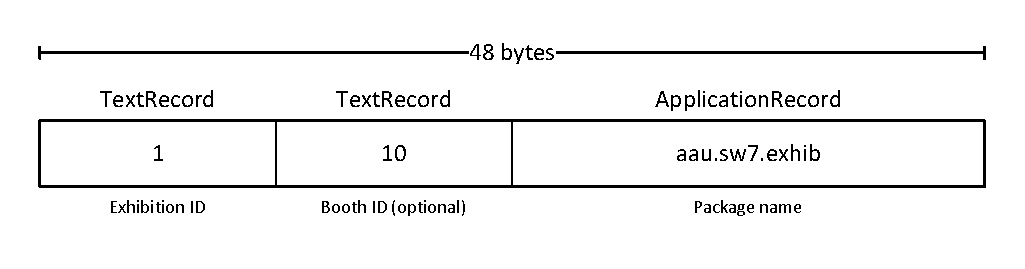
\includegraphics[width=\columnwidth]{img/nfctag.pdf}
\caption{NFC tag message}
\label{fig:nfcdata}
\end{figure}
